\documentclass{article}

\usepackage[utf8]{inputenc}
\usepackage[a4paper, total={6.3in, 8.8in}]{geometry}
\usepackage{amsmath}
\usepackage{bm}
\usepackage{amsfonts}
\usepackage{graphicx}
\usepackage{amssymb}  % assumes amsmath package installed
\usepackage{graphics} % for pdf, bitmapped graphics files
\usepackage{caption}
\usepackage{subcaption}
\usepackage{todonotes}
\usepackage{float}
\usepackage{titling}
\newcommand{\subtitle}[1]{%
  \posttitle{%
    \par\end{center}
    \begin{center}\large#1\end{center}
    \vskip0.5em}%
}


\title{Exercise Session 1: Classification}
\subtitle{Support Vector Machines - Final Report}
\author{Victor van Wymeersch - R0690930}
\date{May 2022}

\begin{document}

\maketitle

\section{Exercises}
    \subsection{Two Gaussian's}
        In this exercise datapoints are generated from two Gaussian distributions with mean of $(1,1)$ and $(-1,-1)$ respectfully. Since the two distributions overlap there is no way to linearly separate the datapoints without some misclassifications, especially when more datapoints are sampled from the distributions as can be seen from figure \ref{fig:two_gaussians}. However, for this dataset an optimal decision boundary can be found through the line $y=-x$ located at the centre between the distributions. 
        % Two gaussians 
        \begin{figure}[h]
            \centering
            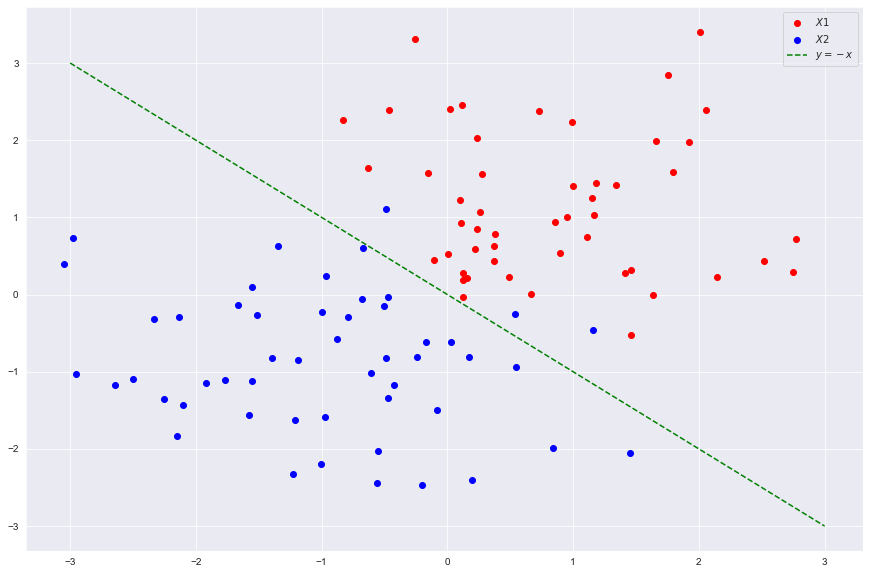
\includegraphics[width=0.5\textwidth]{Assignment 1/figures/two_gaussians.png}
            \caption{Classification boundary between two Gaussian distributions. }
            \label{fig:two_gaussians}
        \end{figure}
    
    \subsection{Support vector machine classifier}
        This exercise involves training a SVM using linear and RBF kernels for classification between datapoints. The effects of increasing the number of samples, and changing regularisation $\gamma$, and bandwidth $\sigma^2$ hyperparameters are investigated. 
        
        \noindent\textbf{Adding datapoints to dataset:}\newline
        When adding datapoints to the dataset different behaviours can be observed depending on the kernel used during classification. Linear kernels can only create linear classification boundaries and thus when datapoints are added to the wrong side of the decision boundary the result is a misclassification. For RBF kernels the the decision boundary shifts to include the new points that was placed on wrong side of the hyperplane. RBF kernels are able to draw nonlinear hyperplanes in the feature space allowing for flexible classifications, however when a datapoint is noise this can result can be a model that does not generalise well, but rather overfits the data. Figure \ref{fig:many_datapoints} shows this phenomenon where the green points located on the red side of are included in the new hyperplane regardless if these points where noise or not. 
        
        % Effect of number of datapoints 
        \begin{figure}[h]
             \centering
             \hspace{0.15\textwidth}
             \begin{subfigure}[b]{0.3\textwidth}
                 \centering
                 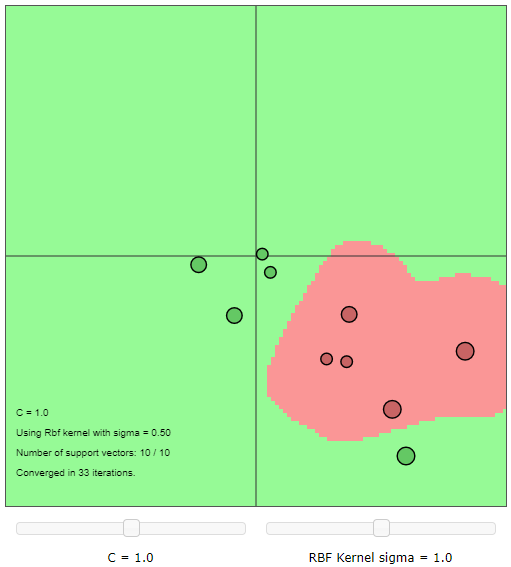
\includegraphics[width=\textwidth]{Assignment 1/figures/RBF_few_datapoints.png}
                 \caption{Few datapoints}
                 \label{fig:few_datapoints}
             \end{subfigure}
             \hfill
             \begin{subfigure}[b]{0.3\textwidth}
                 \centering
                 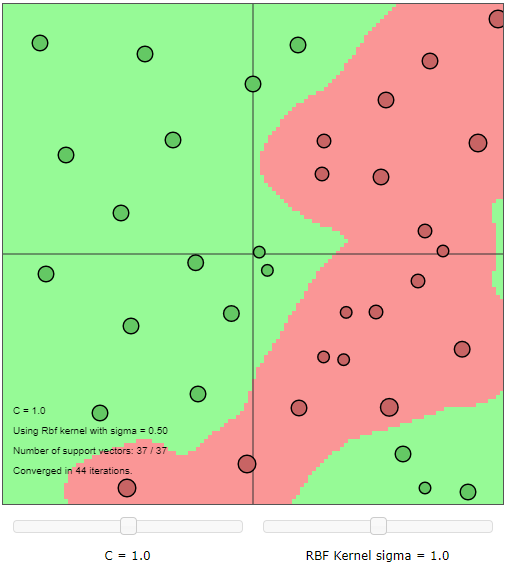
\includegraphics[width=\textwidth]{Assignment 1/figures/RBF_many_datapoints.png}
                \caption{Many datapoints}
                 \label{fig:many_datapoints}
             \end{subfigure}
             \hspace{0.15\textwidth}
            \caption{Effect of increasing the number of datapoints on the classification boundary.}
        \end{figure}
        
        Figure \ref{fig:linearvsrbf} shows the misclassifications that can occur when using a linear kernel and the ability of the non-linear RBF kernel at drawing complex hyperplanes to split the data. For complex datasets RBF kernels generally perform better than linear kernels. 
        % Linear vs RBF kernel 
        \begin{figure}[h]
            
             \centering
             \hspace{0.15\textwidth}
             \begin{subfigure}[b]{0.3\textwidth}
                 \centering
                 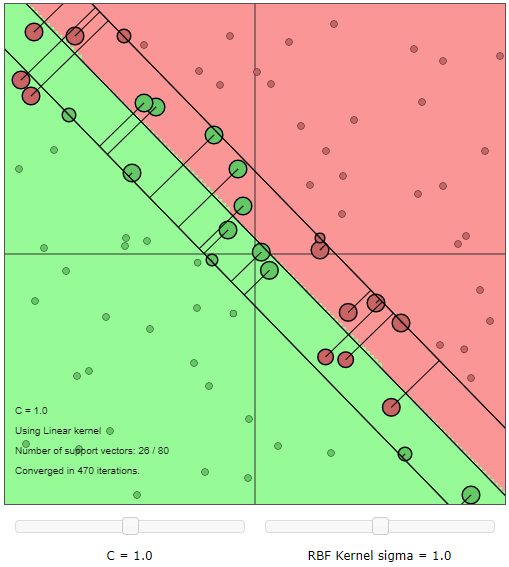
\includegraphics[width=\textwidth]{Assignment 1/figures/linear_vs_rbf_1.png}
                 \caption{Linear kernel}
                 \label{fig:linear_kernel_vs_rbf_1}
             \end{subfigure}
             \hfill
             \begin{subfigure}[b]{0.3\textwidth}
                 \centering
                 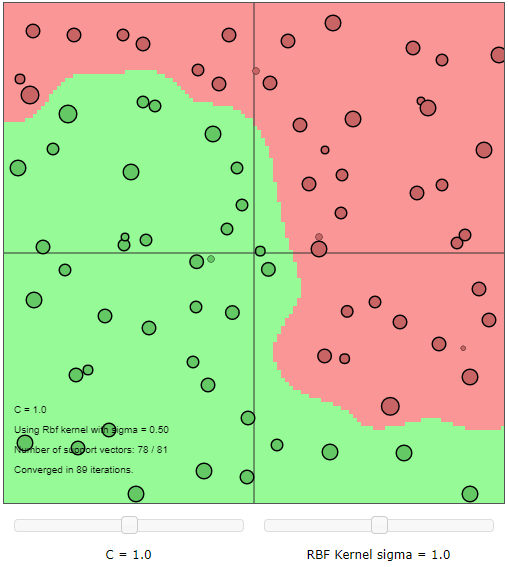
\includegraphics[width=\textwidth]{Assignment 1/figures/linear_vs_rbf_2.png}
                 \caption{RBF kernel}
                 \label{fig:linear_kernel_vs_rbf_2}
             \end{subfigure}
             \hspace{0.15\textwidth}
            \caption{Linear vs. RBF kernel classification problem. }
            \label{fig:linearvsrbf}
        \end{figure}
        
        
        \noindent\textbf{Effect of $\sigma^2$ and $\gamma$ hyperparameters:}\newline 
        Hyperparameter $\gamma$ or in this case C, controls the amount of regularisation in the SVM. C essentially controls the tradeoff between fitting the data and generalising well. As can be seen in figure \ref{fig:rbf_low_regularisation}, when C is small datapoints located on the wrong side of the hyperplane are not considered. However, when C increases in figure \ref{fig:rbf_high_regularisation} a decision boundary forms around the green datapoint because more importance has been placed on the fitting of datapoints. 
        When considering linear kernels the hyperparameter C effects the optimisation by change the slack variables of the optimsation $\xi$. 
        \begin{equation}\label{eq:linearkernel}
        \begin{split}
            \min_{w,b,\xi} & \ \frac{1}{2} w^T w + C \sum^N_{k=1} \xi_k \\
            \text{s.t.} & \ y_k(w^T \varphi(x_k) + b)\geq 1 - \xi_k \\ 
                &\xi_k \geq 0
        \end{split}
        \end{equation}
        
        % Effect of regularisation parameter
        \begin{figure}[h]
             \centering
             \hspace{0.15\textwidth}
             \begin{subfigure}[b]{0.3\textwidth}
                 \centering
                 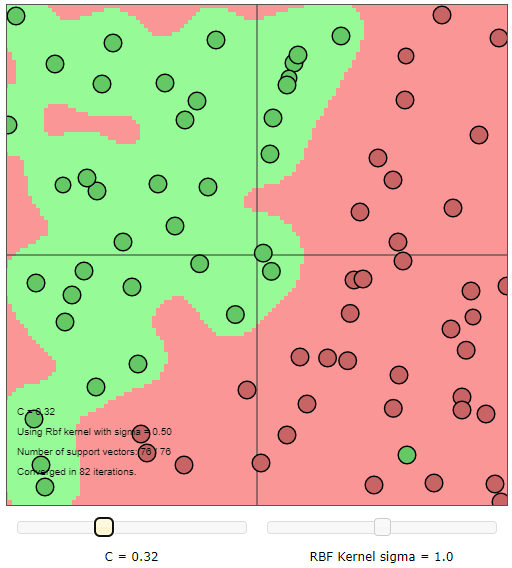
\includegraphics[width=\textwidth]{Assignment 1/figures/RBF_low_regularisation.png}
                 \caption{$C = 0.32$}
                 \label{fig:rbf_low_regularisation}
             \end{subfigure}
             \hfill
             \begin{subfigure}[b]{0.3\textwidth}
                 \centering
                 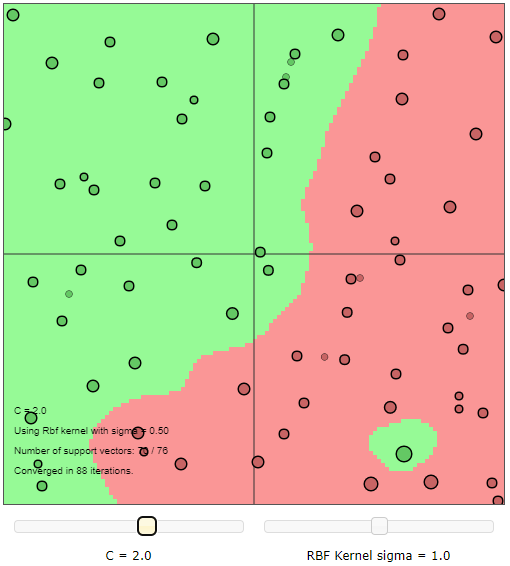
\includegraphics[width=\textwidth]{Assignment 1/figures/RBF_high_regularisation.png}
                 \caption{$C = 2$}
                 \label{fig:rbf_high_regularisation}
             \end{subfigure}
             \hspace{0.15\textwidth}
            \caption{Effect of the regularisation hyperparameter $C$ on the decision boundary.}
        \end{figure}
        
        Hyperparameter $\sigma^2$ refers to the bandwidth of the SVM and has a strong influence on the determination of the decision boundary. As $\sigma$ increases, decisions surfaces become more nonlinear as follows from the definition of the RBF Kernel function: 
        \begin{equation}
            K(x,x') = \exp (-||(x-x_k)||_2^2 / \sigma^2)
        \end{equation}
        Figure \ref{fig:low_sigma} demonstrates overfitting and highly nonlinear decision boundaries that occur when $\sigma$ is chosen as a very small value. Conversely, figure \ref{fig:high_sigma} shows the linear decision boundary created when $\sigma$ is chosen as a large value. Generally this parameter is chosen based on the problem at hand and can be tuned though various methods such as Gridsearch. 
        % Effect of sigma2 values  
        \begin{figure}[h]
             \centering
             \begin{subfigure}[b]{0.3\textwidth}
                 \centering
                 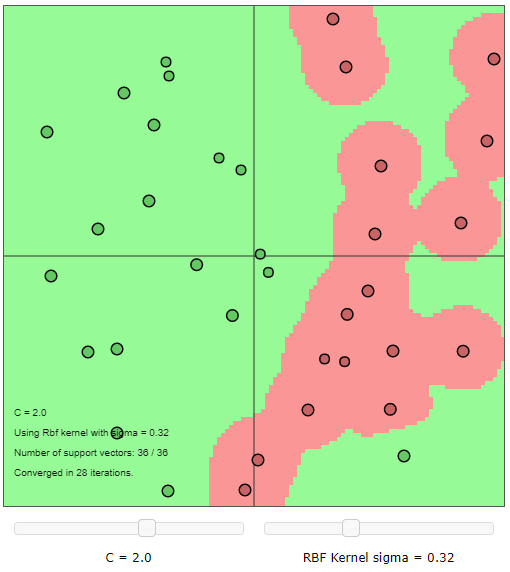
\includegraphics[width=\textwidth]{Assignment 1/figures/RBF_low_sigma.png}
                 \caption{$\sigma^2 = 0.32$}
                 \label{fig:low_sigma}
             \end{subfigure}
             \hfill
             \begin{subfigure}[b]{0.3\textwidth}
                 \centering
                 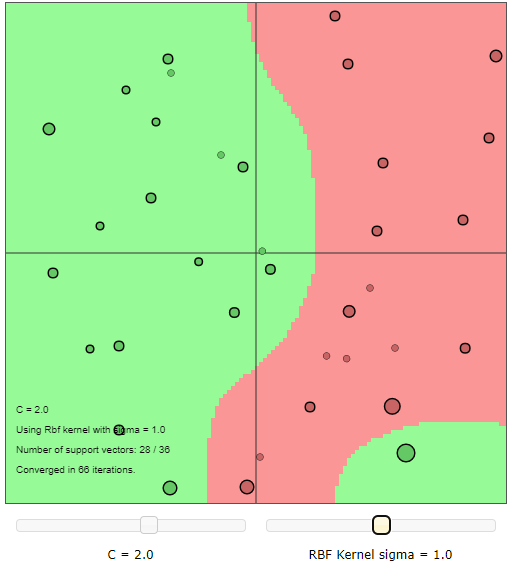
\includegraphics[width=\textwidth]{Assignment 1/figures/RBF_medium_sigma.png}
                 \caption{$\sigma^2 = 1.0$}
                 \label{fig:medium_sigma}
             \end{subfigure}
             \hfill
             \begin{subfigure}[b]{0.3\textwidth}
                 \centering
                 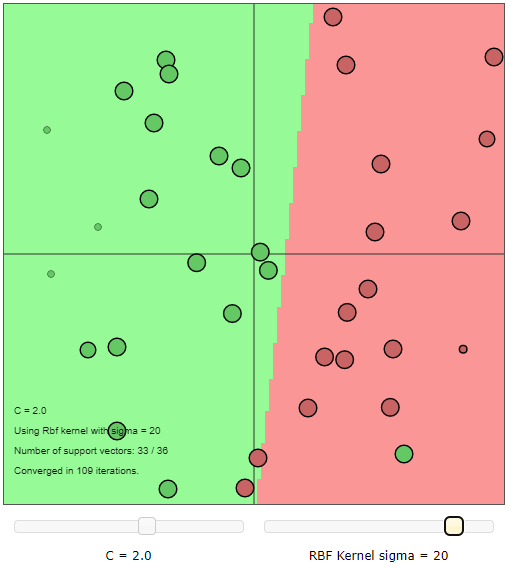
\includegraphics[width=\textwidth]{Assignment 1/figures/RBF_high_sigma.png}
                 \caption{$\sigma^2 = 20$}
                 \label{fig:high_sigma}
             \end{subfigure}
            \caption{Effect of increasing $\sigma^2$ hyperparameter on the decision boundary.}
        \end{figure}
        
        
    \subsection{Least-squares support vector machine classifier}
        This section concerns binary classification on the Iris dataset. The influence of different kernel choices and hyperparameters are discussed.
        
        \subsubsection{Influence of hyperparameters and kernel parameters}
           Polynomial kernels functions allow for both linear and nonlinear classification boundaries. The polynomial degree of a polynomial kernel influences how nonlinear the decision boundary can become, and in this sense serves a similar function as that of the $\sigma^2$ parameter of RBF kernels. When the polynomial degree is $1$ only linear boundaries can be made. Figure \ref{fig:polynomial_degree} shows the classification accuracy for increasing polynomial degrees on the test set. As the polynomial degree increases the classifier is able to draw more nonlinear hyperplanes through the feature space resulting in better classification accuracy's. Although the figure suggests that larger polynomial degrees always result in better classification accuracy, a too high degree can cause overfitting of the data. 
           
           Figure \ref{fig:rbf_sigma2} demonstrates the effect of $\sigma^2$ on the classification accuracy on the test set. A reasonable choice for $\sigma^2$ on the Iris dataset is simply $0$. A good choice for the regularisation parameter $\gamma$ can be chosen in  a similar fashion to $\sigma^2$, with too small values resulting in over-regularisation and poor classification accuracy due to an inability to fit the data. More comprehensive parameter sweeps for $\sigma^2$ and the regularisation parameter $\gamma$ on the Iris dataset can be observed in the next section. 
            % Effect of hyperparameters 
            \begin{figure}[h]
                 \centering
                 \hspace{0.05\textwidth}
                 % Polynomial degree
                 \begin{subfigure}[b]{0.4\textwidth}
                     \centering
                     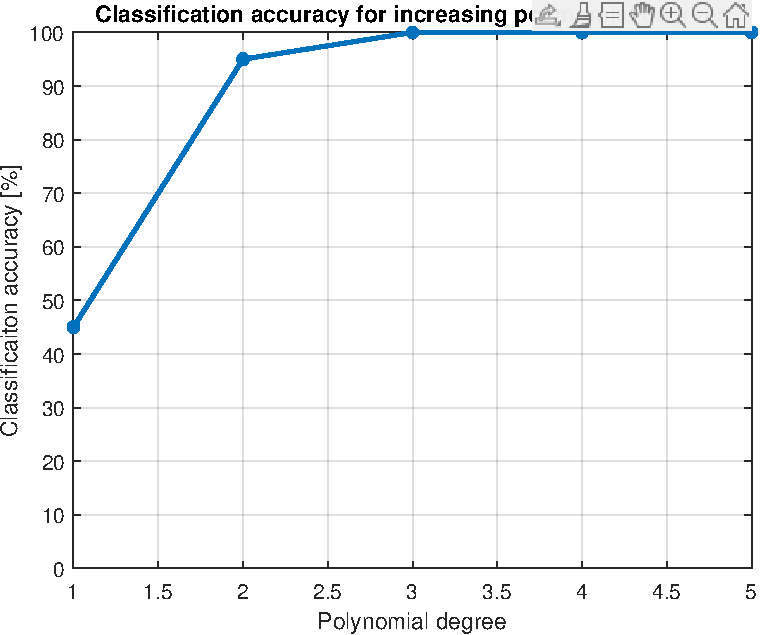
\includegraphics[width=\textwidth]{Assignment 1/figures/class_acc_poly_deg_val.pdf}
                    \caption{Varying polynomial degree}
                     \label{fig:polynomial_degree}
                 \end{subfigure}
                 \hfill
                 % RBF sigma2 
                 \begin{subfigure}[b]{0.4\textwidth}
                     \centering
                     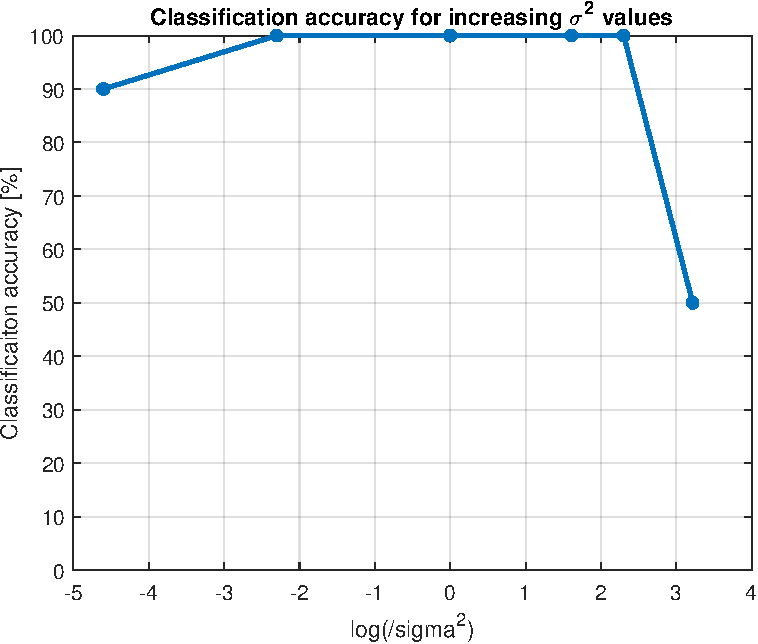
\includegraphics[width=\textwidth]{Assignment 1/figures/class_acc_sigma2_val.pdf}
                    \caption{Varying $\sigma^2$}
                     \label{fig:rbf_sigma2}
                 \end{subfigure}
                 \hspace{0.05\textwidth}
                \caption{Effect of varying polynomial degree (a) and $\sigma^2$ (b) on classification accuracy. }
            \end{figure}
            
        % Tuning for Gamma and Sigma is done in the next section - just explain and point here 
            
        \subsubsection{Tuning parameters using validation}
            This section covers comprehensive Gridsearch parameter sweeps for $\gamma$ and $\sigma^2$ over three different validation schemes, namely Random split, k-fold cross-validation and leave-one-out validation. Each parameter tested in the gridsearch is evaluated and their percentage misclassification costs are plotted as surface plots. 
            
            \noindent \textbf{Random split}: \newline
            The random split validation technique splits the data randomly into a training and a validation set. Here the training data is used to train the model and the validation data is used to evaluate the performance of the model. Figure \ref{fig:random_split_validation} shows the misclassification cost for this method for all the tested values of $\gamma$ and $\sigma^2$. Several choices for the hyperparameters yield a 0 misclassification cost and seem to have a very good performance. However, it can be noticed that the surface plot is quite jagged and should be noted that some random validation splits may not accurately represent the training data after sampling.
            
            
            \noindent \textbf{k-fold cross validation}: \newline
            K-fold cross validation splits the data into k subsets. K-1 of these subsets are used for training of the model and one is used for validation. The process is repeated for all combinations of the training and validation subsets. The misclassification error over all of the folds are evaluated and the average is taken as the final error. Figure \ref{fig:10_fold_validation} shows the average misclassifcation error over 10 folds. This method is not susceptible to the same sampling issues as a standard random split, resulting in a smoother surface plot and more robust hyperparameter values. 
            
            \noindent \textbf{Leave-one-out validation}: \newline
            Leave-one-out validation follows the same principle as k-fold cross validation, with the only difference being that N-1 samples are used for training and only a single for validation. The result of this validation technique is shown in figure \ref{fig:loo_validation}. The results of this validation technique is most robust compared to the other validation techniques, and the optimal values for $\sigma^2$ and $\gamma$ for leave-one-out cross validation are more likely to perform well on test sets. The drawback of leave-one-out cross validation requires many more evaluations  have to be performed when compared to the other validation techniques. This drastically increases the computational time required for such tuning. 
            
            In many cases 10-fold cross validation strikes a good balance between computational demand and robustly tuned hyperparmeters. 
            
            
            % Hyperparameter tuning for different validation techniques
            \begin{figure}[h]
             \centering
             \begin{subfigure}[b]{0.45\textwidth}
                 \centering
                 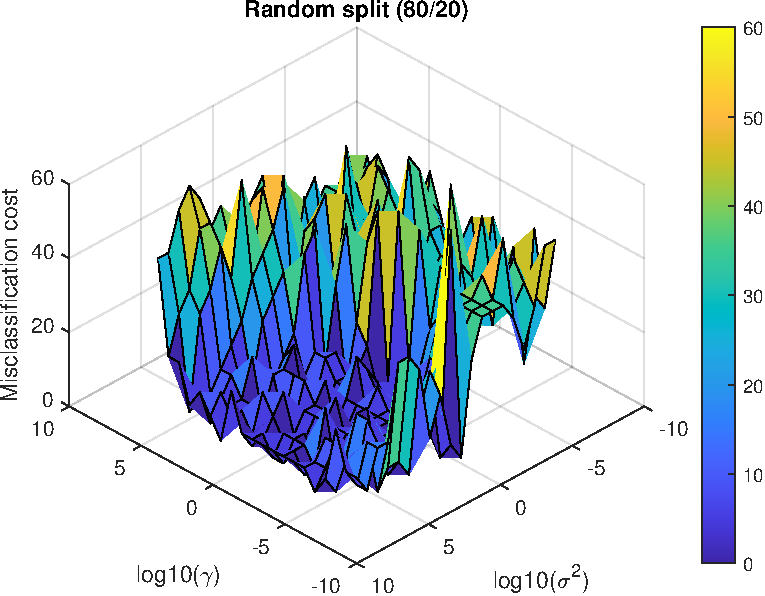
\includegraphics[width=\textwidth]{Assignment 1/figures/random_split_validation_surf.pdf}
                \caption{}
                 \label{fig:random_split_validation}
             \end{subfigure}
             \hfill
             \begin{subfigure}[b]{0.45\textwidth}
                 \centering
                 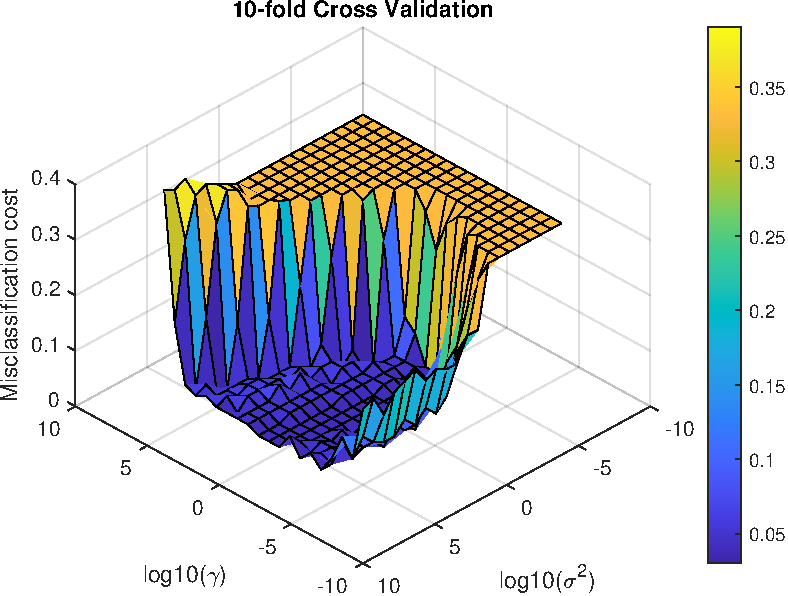
\includegraphics[width=\textwidth]{Assignment 1/figures/10_fold_cross_validation_surf.pdf}
                \caption{}
                 \label{fig:10_fold_validation}
             \end{subfigure}
             \hfill
             \begin{subfigure}[b]{0.45\textwidth}
                 \centering
                 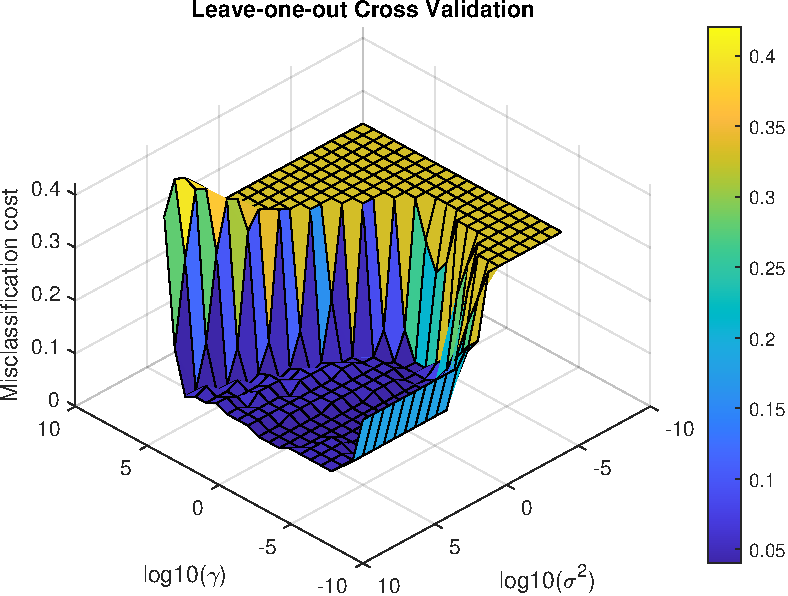
\includegraphics[width=\textwidth]{Assignment 1/figures/loo_cross_validation_surf.pdf}
                \caption{}
                 \label{fig:loo_validation}
             \end{subfigure}
            \caption{Effect of $\sigma^2$ and $\gamma$ hyperparameters on cost minimisation for different validation techniques. }
        \end{figure}
            
            
        \subsubsection{Automatic parameter tuning}
            The tuning of SVMs can be automated using algorithmic tuning techniques such as Simplex or Gridsearch. These methods both utilise Coupled Simulated Annealing (CSA) as an initial point for their optimisation. 
            
            CSA uses a temperature parameter to control the production of solutions, lowering it over time to minimise its cost function. The result of CSA is an approximation of the global optimum, but because CSA is a probabilistic algorithm the initial estimate can vary between runs. The Simplex and Gridsearch methods leverage the initial estimate to speed up the time required for hyperparameter tuning. The results of these two algorithms are outlined in table \ref{tab:gridsimp}. 
            
            \begin{table}[]
            
            \centering
            \begin{tabular}{|c|c|c|}
            \hline
            \multicolumn{1}{|l|}{} & \textbf{Simplex} & \textbf{Gridsearch} \\ \hline
            $\gamma$               & 0.07             & 17.24               \\ \hline
            $\sigma^2$             & 1.8              & 0.08                \\ \hline
            CPU time               & 2.78             & 3.69                \\ \hline
            \end{tabular}
            \caption{Results of Simplex and Gridsearch algorithmic hyperparameter tuning.}
            \label{tab:gridsimp}
            \end{table}
            
            The Gridsearch algorithm performs an exhaustive search around the initial point provided by the CSA algorithm. This exhaustive search is why the CPU time of the Gridsearch method is higher than that of the Simplex method. However, both methods are able to fine good sets of hyperparameters for the classification task as can be seen in figure \ref{fig:searchmethods}. 
            
            % Simplex and gridsearch hyperparameter tuning results 
            \begin{figure}[h]
                
                 \centering
                 \hspace{0.05\textwidth}
                 % Simplex
                 \begin{subfigure}[b]{0.4\textwidth}
                     \centering
                     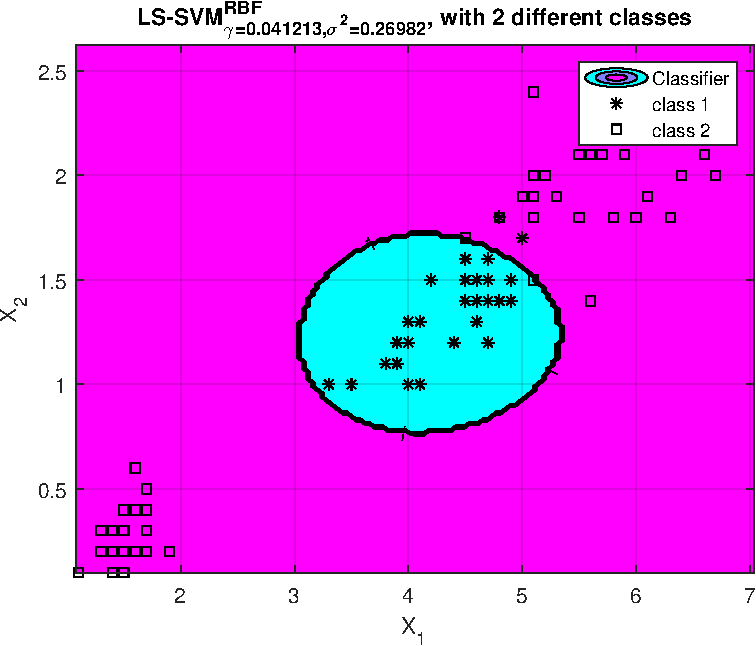
\includegraphics[width=\textwidth]{Assignment 1/figures/rbf_simplex_optimal.pdf}
                    \caption{Simplex algorithm}
                     \label{fig:rbf_simplex_tuned}
                 \end{subfigure}
                 \hfill
                 % Gridsearch
                 \begin{subfigure}[b]{0.4\textwidth}
                     \centering
                     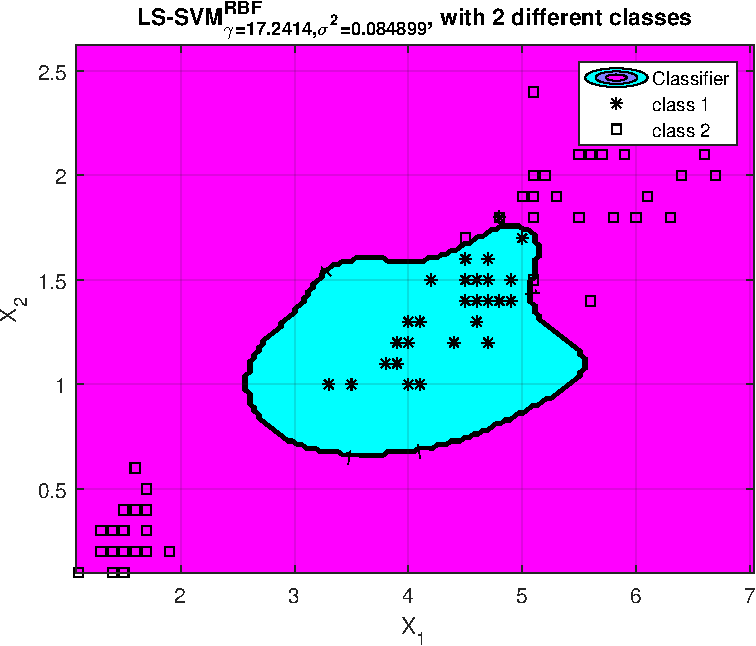
\includegraphics[width=\textwidth]{Assignment 1/figures/rbf_gridsearch_optimal.pdf}
                    \caption{Gridsearch algorithm}
                     \label{fig:rbf_gridsearch_tuned}
                 \end{subfigure}
                 \hspace{0.05\textwidth}
                \caption{Classification results for RBF kernels tuned using Simplex (a) and Gridsearch (b) algorithms.}
                \label{fig:searchmethods}
            \end{figure}
            
        \subsubsection{Using ROC curves}
            Receiver Operative Characteristic (ROC) curves show the separation abilities of binary classifiers. They are created by plotting True Positive (TP) and False Positive (FP) rates against each other for various different classifier thresholds. The result is a plot whose area under the curve represents the discriminative power of a classifier. 
            
            Figure \ref{fig:roc_curves_all} shows the ROC curves for a RBF kernel SVM tuning with Simplex and Gridsearch methods, and Linear kernel SVM. It can be seen that both RBF kernel models are able to perfectly classify the test set, where the linear model is unable to. We use the test set rather than the training set to ensure that data used to train the model is not used to also evaluate the model as this would give a biased performance of the classifier. 
            
             % Linear vs RBF simplex vs RBF gridsearch ROC curves
            \begin{figure}[h]
            
                 \centering
                 % Simplex RBF
                 \begin{subfigure}[b]{0.3\textwidth}
                     \centering
                     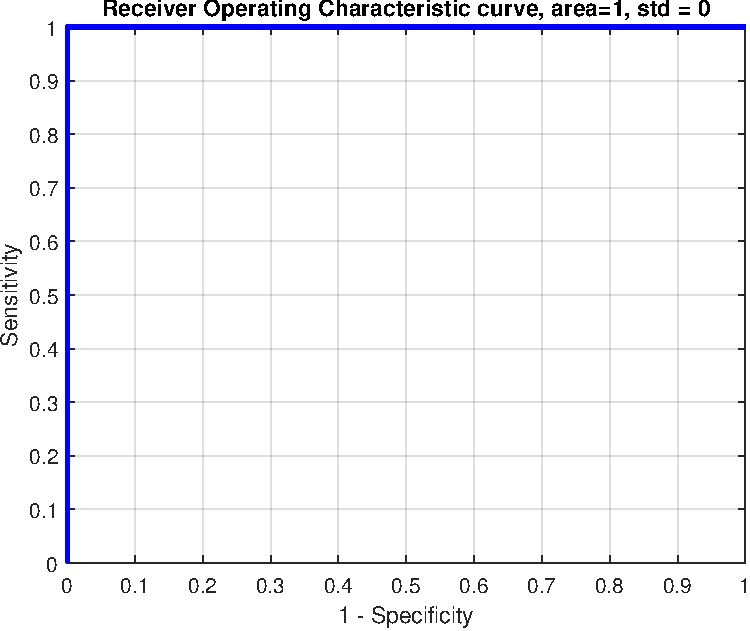
\includegraphics[width=\textwidth]{Assignment 1/figures/simplex_rbf_classifier_roc.pdf}
                    \caption{RBF Simplex}
                     \label{fig:roc_rbf_simplex_tuned}
                 \end{subfigure}
                 \hfill
                 % Gridsearch RBF
                 \begin{subfigure}[b]{0.3\textwidth}
                     \centering
                     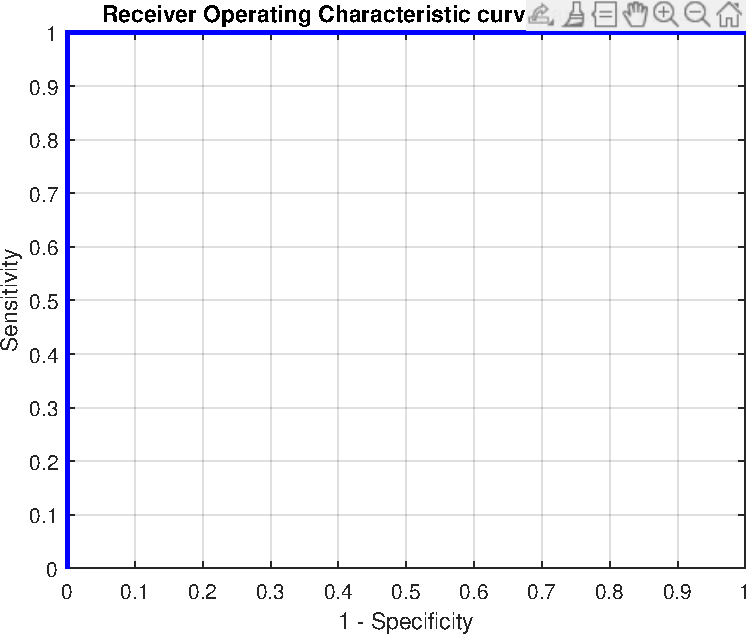
\includegraphics[width=\textwidth]{Assignment 1/figures/gridsearch_rbf_classifier_roc.pdf}
                    \caption{RBF Gridsearch}
                     \label{fig:roc_rbf_gridsearch_tuned}
                 \end{subfigure}
                 \hfill
                 % linear 
                 \begin{subfigure}[b]{0.3\textwidth}
                     \centering
                     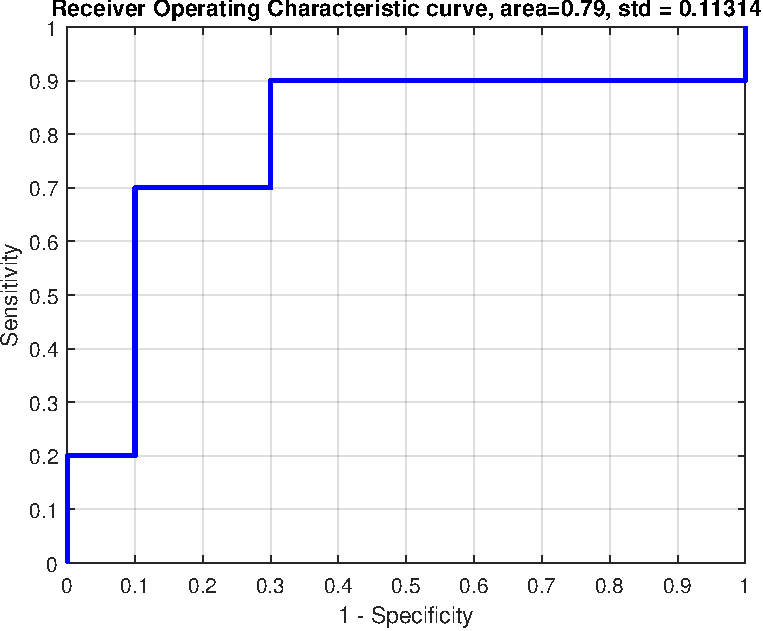
\includegraphics[width=\textwidth]{Assignment 1/figures/linear_classifier_roc.pdf}
                    \caption{Linear}
                     \label{fig:roc_linear}
                 \end{subfigure}
                \caption{ROC curves for Simplex- (a), Gridsearch-tuned RBF (b), and linear kernels (c). }
                \label{fig:roc_curves_all}
            \end{figure}
            
        
        \subsubsection{Bayesian framework} 
            Using a Bayesian framework it is possible to get probability estimates. These probability estimates are then used to calculate the posterior class probabilities of a datapoint belonging to a class given the uncertainty of the parameters. 
            
            Figures \ref{fig:bayes_fig_sigma} and \ref{fig:bayes_fig_gamma} show the classification results on the Iris dataset within the Bayesian framework for different values of $\sigma^2$ and $\gamma$. The colours of the plot represent the probability of a sample belonging to the positive class, with pink and blue representing 100\% and 0\% probabilities, respectfully. 
            
            Figure \ref{fig:bayes_fig_sigma} shows how the kernel bandwidth $\sigma^2$ influences the results of the classifications. For larger values of sigma the area of influence of the positive datapoints shrinks and the area of influence of the negative samples increases. 
            
            % Bayesian Sigma2 tuning figures 
            \begin{figure}[h]
                 \centering
                 
                 \begin{subfigure}[b]{0.3\textwidth}
                     \centering
                     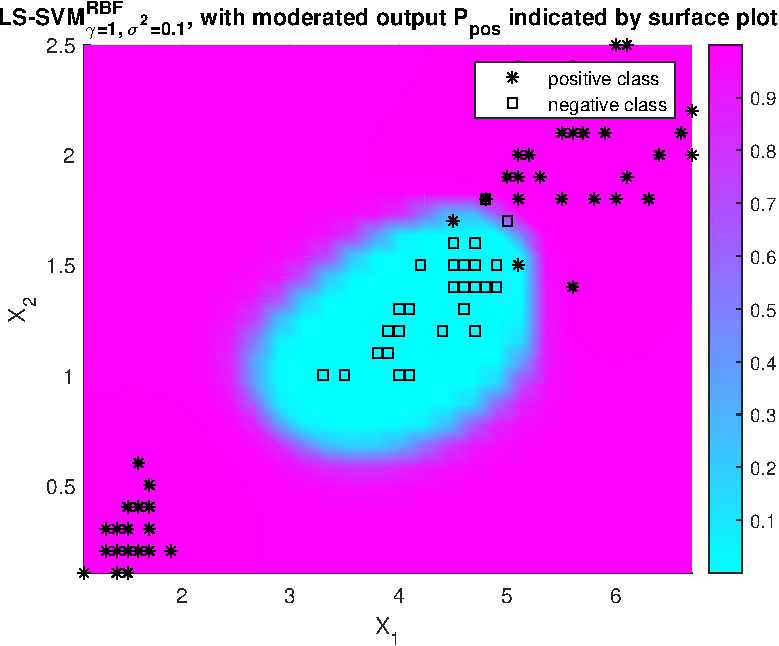
\includegraphics[width=\textwidth]{Assignment 1/figures/bayes_rbf_gamma_1_sig2_1.000000e-01}
                    \caption{$\gamma = 1, \ \sigma^2 = 0.1$}
                     \label{fig:bayes_1}
                 \end{subfigure}
                 \hfill
                 \begin{subfigure}[b]{0.3\textwidth}
                     \centering
                     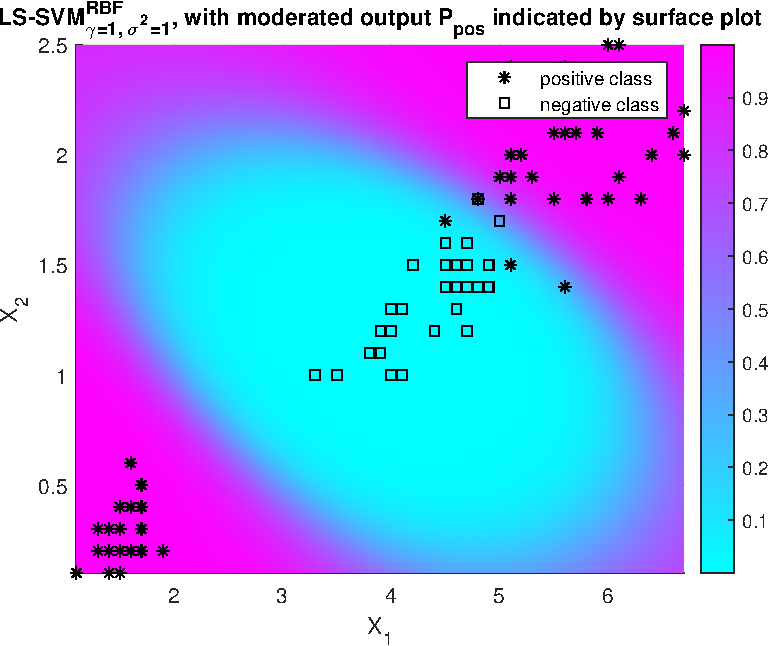
\includegraphics[width=\textwidth]{Assignment 1/figures/bayes_rbf_gamma_1_sig2_1.pdf}
                    \caption{$\gamma = 1, \ \sigma^2 = 1$}
                     \label{fig:bayes_2}
                 \end{subfigure}
                 \hfill
                 \begin{subfigure}[b]{0.3\textwidth}
                     \centering
                     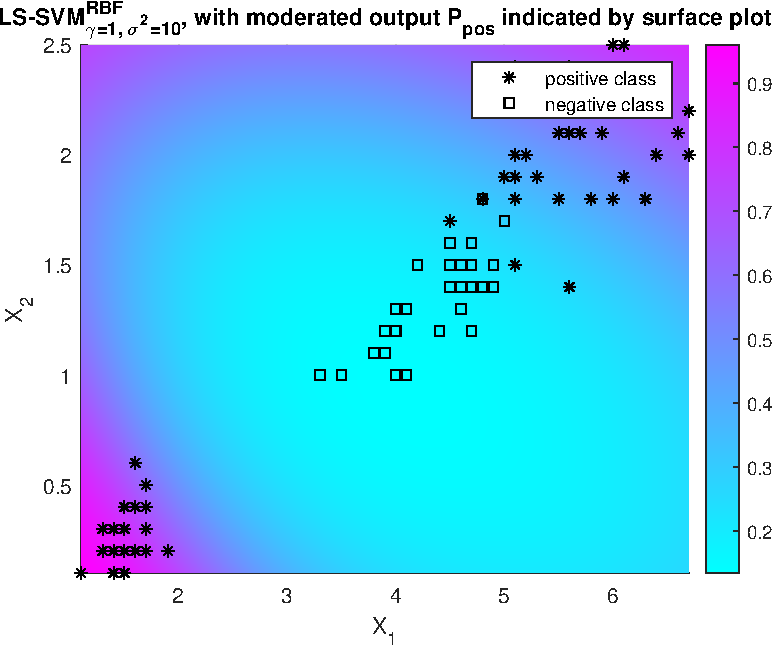
\includegraphics[width=\textwidth]{Assignment 1/figures/bayes_rbf_gamma_1_sig2_10.pdf}
                    \caption{$\gamma = 1, \ \sigma^2 = 10$}
                     \label{fig:bayes_3}
                 \end{subfigure}
                \caption{Bayesian SVM classification results for varying $\sigma^2$ values.}
                \label{fig:bayes_fig_sigma}
            \end{figure}
            
            Figure \ref{fig:bayes_fig_gamma} shows how the regularisation $\gamma$ influences the results of the classifications. For larger values of gamma the certainty the model has about a point belonging to the positive class decreases from 1.0 when $\gamma = 0.01$ to a maximum of $~0.75$ when $\gamma=10$. Essentially the additional smoothing of the regularisation parameter increases the uncertainty of the model resulting in a smoother decision boundary. 
            
            % Bayesian Gamma tuning figures 
            \begin{figure}[h]
            
                 \centering
                 \begin{subfigure}[b]{0.3\textwidth}
                     \centering
                     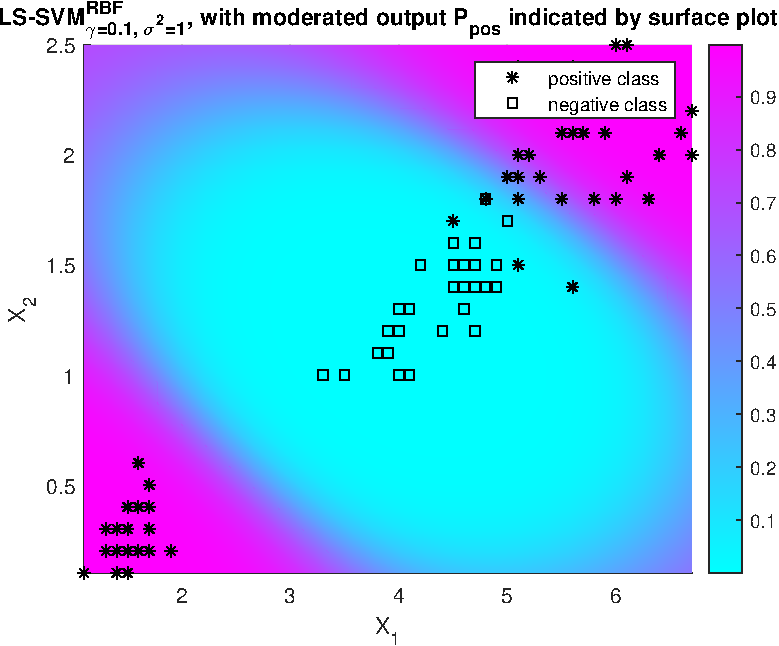
\includegraphics[width=\textwidth]{Assignment 1/figures/bayes_rbf_gamma_1.000000e-01_sig2_1.pdf}
                    \caption{$\gamma =0.01,/ \sigma^2 = 1$}
                     \label{fig:bayes_4}
                 \end{subfigure}
                 \hfill
                 \begin{subfigure}[b]{0.3\textwidth}
                     \centering
                     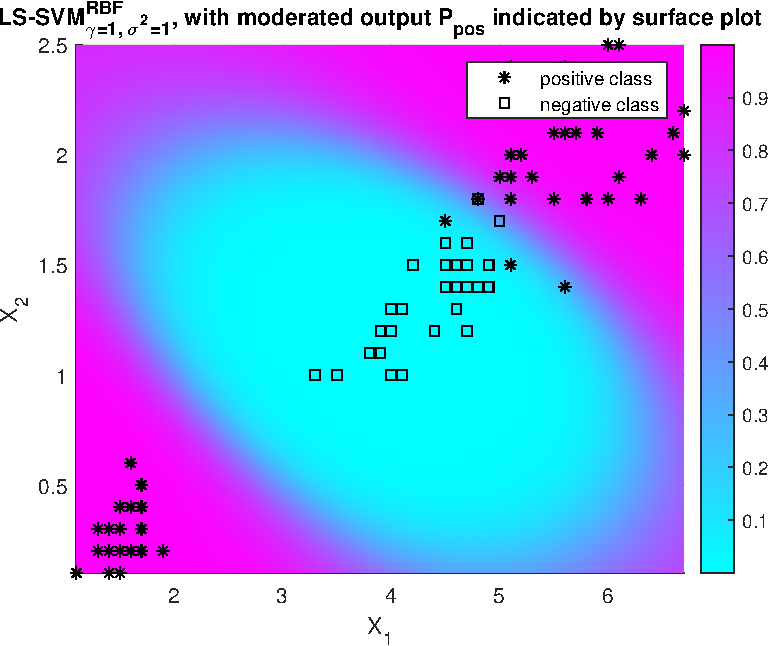
\includegraphics[width=\textwidth]{Assignment 1/figures/bayes_rbf_gamma_1_sig2_1.pdf}
                    \caption{$\gamma = 1,/ \sigma^2 = 1$}
                     \label{fig:bayes_5}
                 \end{subfigure}
                 \hfill
                 \begin{subfigure}[b]{0.3\textwidth}
                     \centering
                     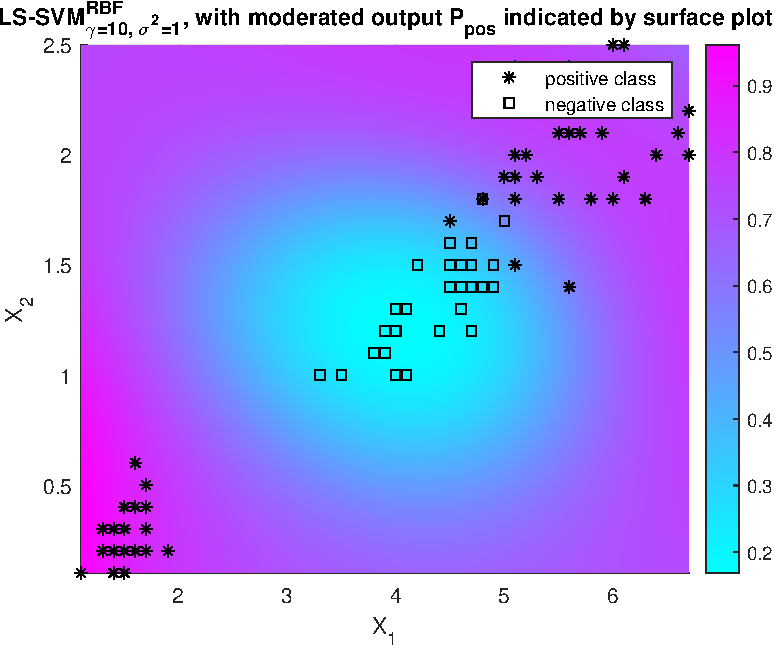
\includegraphics[width=\textwidth]{Assignment 1/figures/bayes_rbf_gamma_10_sig2_1.pdf}
                    \caption{$\gamma = 10,/ \sigma^2 = 1$}
                     \label{fig:bayes_6}
                 \end{subfigure}
                \caption{Bayesian SVM classification results for varying amounts of regularisation, $\gamma$.}
                \label{fig:bayes_fig_gamma}
            \end{figure}
        
\section{Homework problems}
    \subsection{Ripley dataset} 
        The Ripley dataset consists of to classes generated by two Gaussian distributions each. The dataset is visualised in figure \ref{fig:ripley_two_gaussians}. The dataset is not linearly separable since the two classes overlap each other. 
        % Ripley dataset 
        \begin{figure}[H]
            \centering
            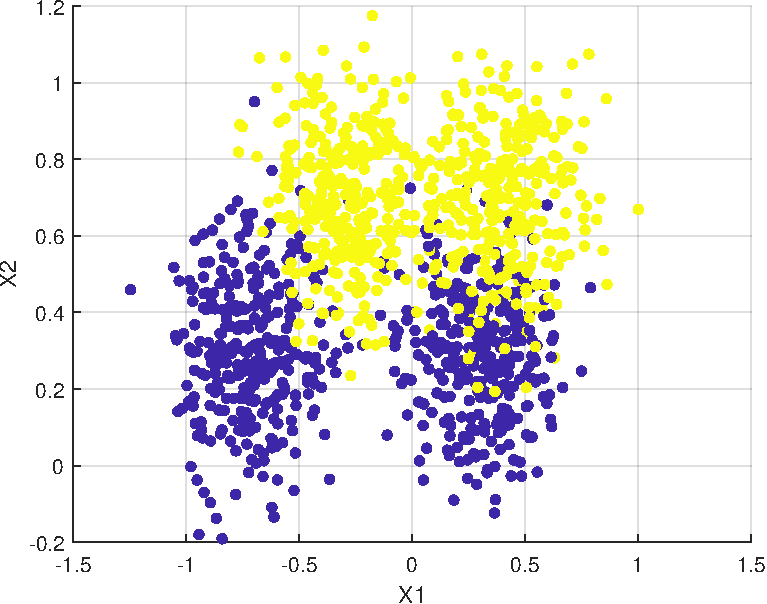
\includegraphics[width=0.450\textwidth]{Assignment 1/figures/ripley_data.pdf}
            \caption{Ripley dataset with shape $(1250,2)$, $\bar{X}_1=-0.07, \bar{X}_2=0.49$ means, and $ \sigma_1=0.48, \sigma_2=0.26$ standard deviations. }
            \label{fig:ripley_two_gaussians}
        \end{figure}
        
        Linear, RBF, and polynomial kernels were tested with Simplex-tuned hyperparameters over a  10-fold cross validation set. The results are shown in figure \ref{fig:ripley_overall}. The best performing classified was the RBF kernel obtaining a ROC curve area of $0.96856$ for hyperparameters $\sigma^2 = 0.65538$ and $\gamma=5.0469$. The performance of this kernel and chosen hyperparameters performs very well on the data and is the preferred choice over a linear kernel as it can effectively capture the split between the Gaussian distributions.  
        
        % Ripley dataset for tuned Linear RBF and poly kernels 
         % Bayesian Gamma tuning figures 
            \begin{figure}[H]
                
                 \centering
                 \begin{subfigure}[b]{0.3\textwidth}
                     \centering
                     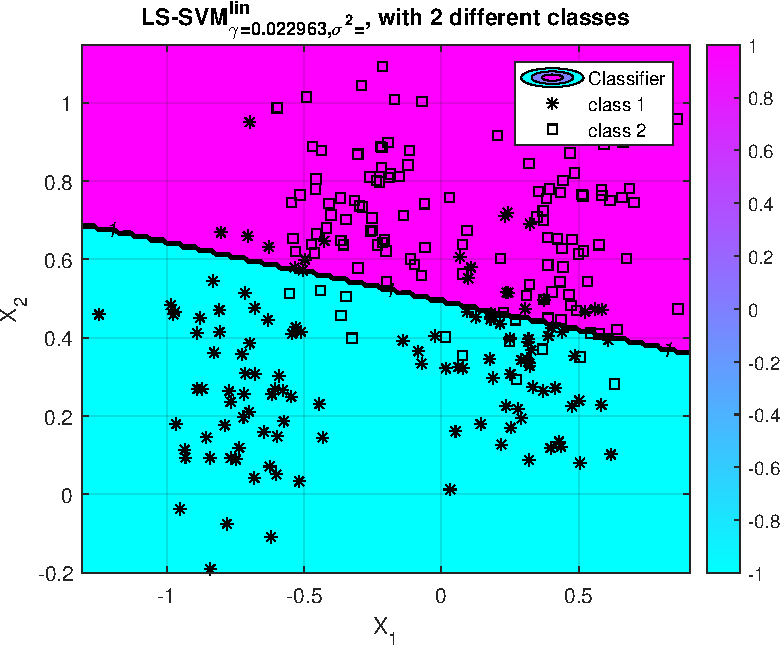
\includegraphics[width=\textwidth]{Assignment 1/figures/ripley_simplex_linear_classification_result.pdf}
                    \caption{Linear kernel}
                     \label{fig:ripley_linear_result}
                 \end{subfigure}
                 \hfill
                 \begin{subfigure}[b]{0.3\textwidth}
                     \centering
                     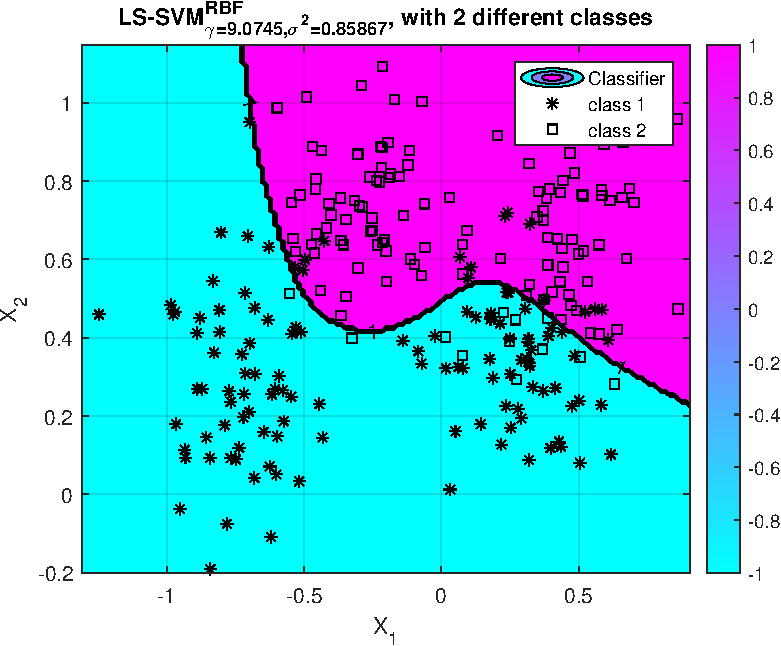
\includegraphics[width=\textwidth]{Assignment 1/figures/ripley_simplex_rbf_classification_result.pdf}
                    \caption{RBF kernel}
                     \label{fig:ripley_rbf_result}
                 \end{subfigure}
                 \hfill
                 \begin{subfigure}[b]{0.3\textwidth}
                     \centering
                     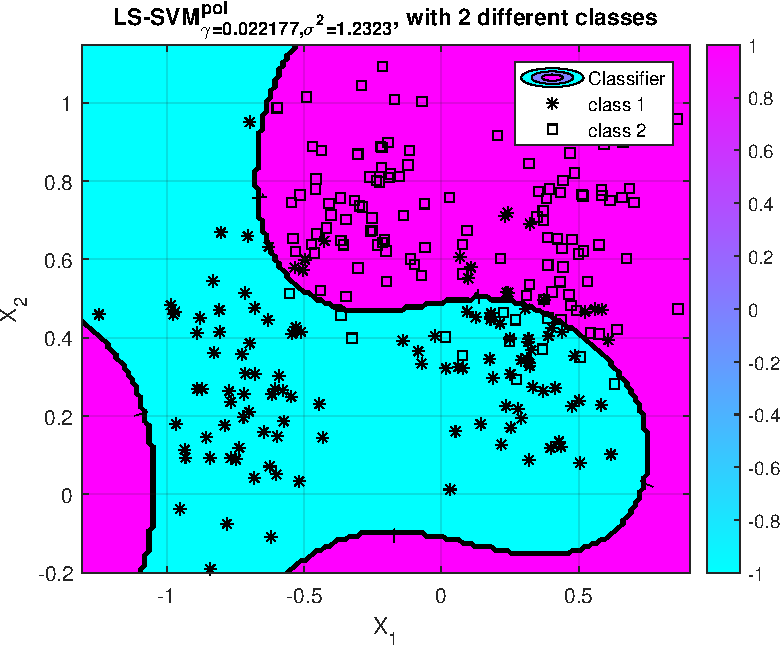
\includegraphics[width=\textwidth]{Assignment 1/figures/ripley_simplex_polynomial_classification_result.pdf}
                    \caption{Polynomial kernel}
                     \label{fig:ripley_poly_result}
                 \end{subfigure}
                 \hfill
                 \begin{subfigure}[b]{0.3\textwidth}
                     \centering
                     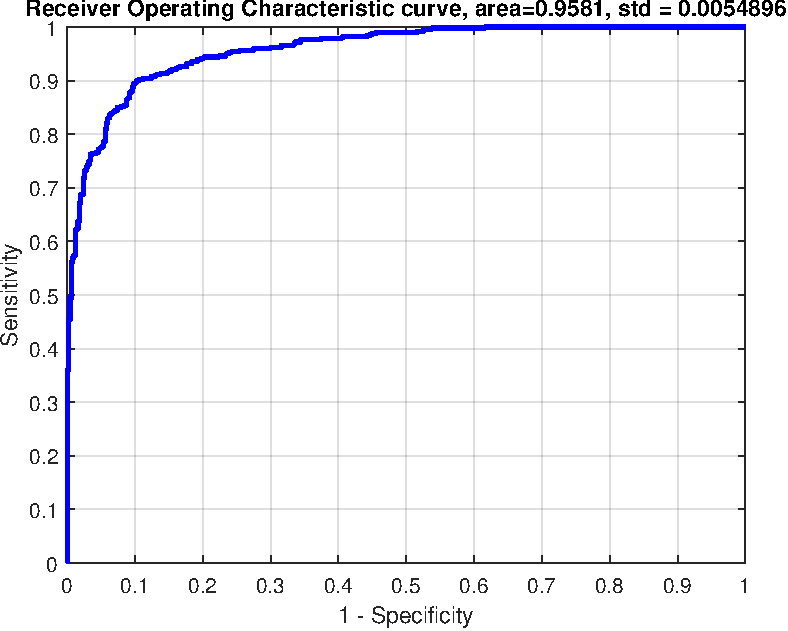
\includegraphics[width=\textwidth]{Assignment 1/figures/ripley_simplex_linear_classifier_roc.pdf}
                    \caption{Linear kernel}
                     \label{fig:ripley_linear_roc}
                 \end{subfigure}
                 \hfill
                 \begin{subfigure}[b]{0.3\textwidth}
                     \centering
                     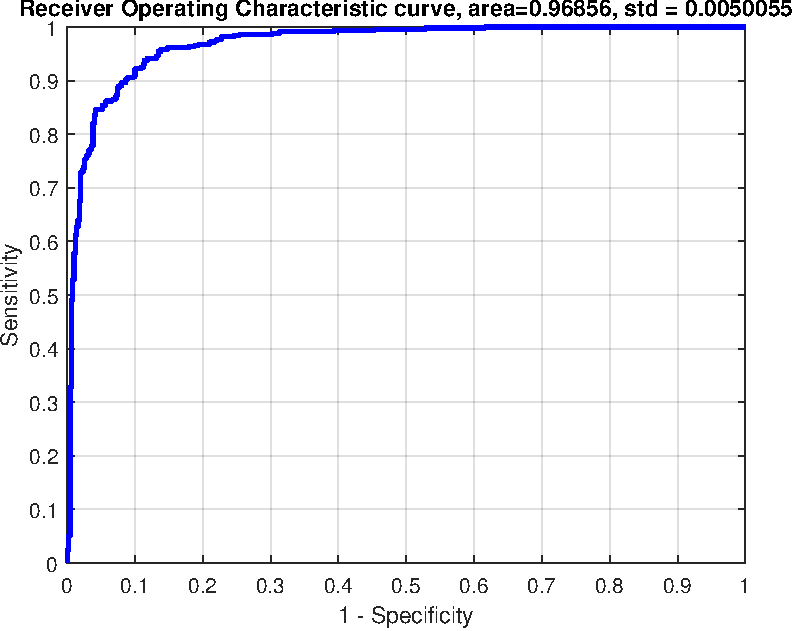
\includegraphics[width=\textwidth]{Assignment 1/figures/ripley_simplex_rbf_classifier_roc.pdf}
                    \caption{RBF kernel}
                     \label{fig:ripley_rbf_roc}
                 \end{subfigure}
                 \hfill
                 \begin{subfigure}[b]{0.3\textwidth}
                     \centering
                     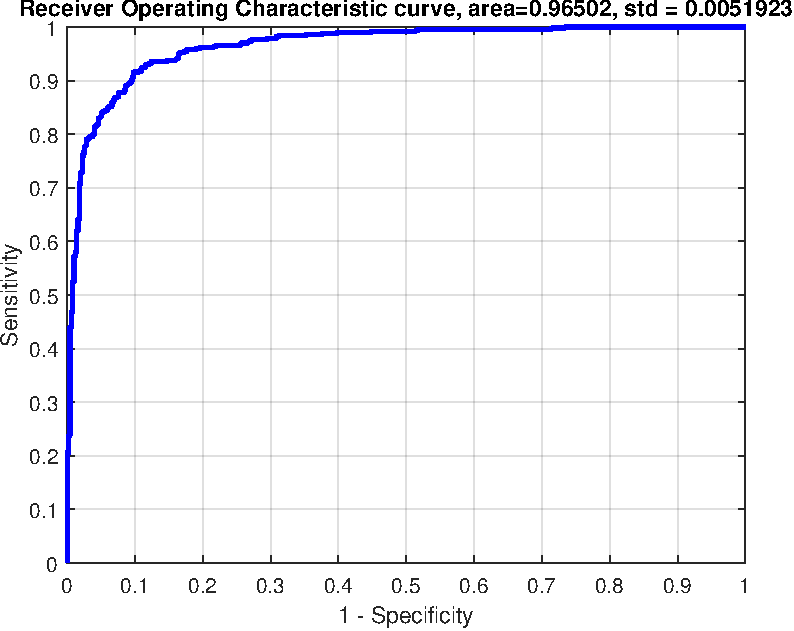
\includegraphics[width=\textwidth]{Assignment 1/figures/ripley_simplex_polynomial_classifier_roc.pdf}
                    \caption{Polynomial kernel}
                     \label{fig:ripley_poly_roc}
                 \end{subfigure}
                \caption{Classification results on the Ripley dataset for linear, RBF and Polynomial kernels tuned with the Simplex algorithm.}
                \label{fig:ripley_overall}
            \end{figure}
        
    \subsection{Wisconsin Breast Cancer dataset}
        The Wisconsin Breast Cancer dataset consists of 569 datapoints and 30 input features. A t-SNE plot was used to visualise the dataset since there are too many features to plot in 2 or 3 dimensions. The t-SNE plot is shown in figure \ref{fig:breast_cancer_dataset}.  
        
        According to Cover's theorem, provided that the feature space is not densly populated, it is more probable that a set is linearly separable in a high dimensional space than that of a low dimensional space. Since, the dataset contains a high dimensional feature space and that the t-SNE plot shows little overlap between features it is probable that a linear kernel SVM classifier will perform fairly well on this dataset. 
        
        % Breast cancer dataset
        \begin{figure}[H]
            \centering
            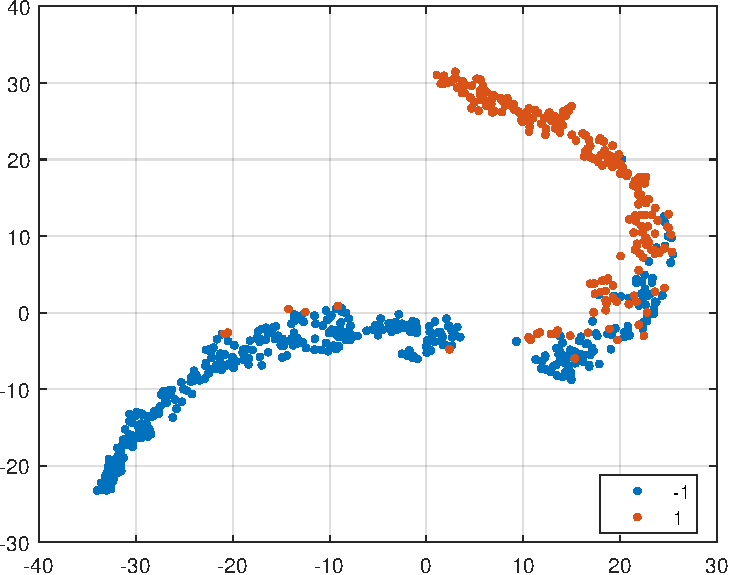
\includegraphics[width=0.450\textwidth]{Assignment 1/figures/breast_data.pdf}
            \caption{Breast cancer dataset with shape $(569,30)$.}
            \label{fig:breast_cancer_dataset}
        \end{figure}
        
        Linear, RBF, and polynomial kernels are evaluated in the same method as for the Ripley dataset, with models being Simplex-tuned over a 10-fold cross validation set. The results of the classifiers are presented in figure \ref{fig:breast_cancer_overall}. As suspected the linear kernel performs very well, almost surpassing the RBF kernel.
        
        % ROC curves for breast cancer dataset 
        \begin{figure}[H]
             \centering
             
             \begin{subfigure}[b]{0.3\textwidth}
                 \centering
                 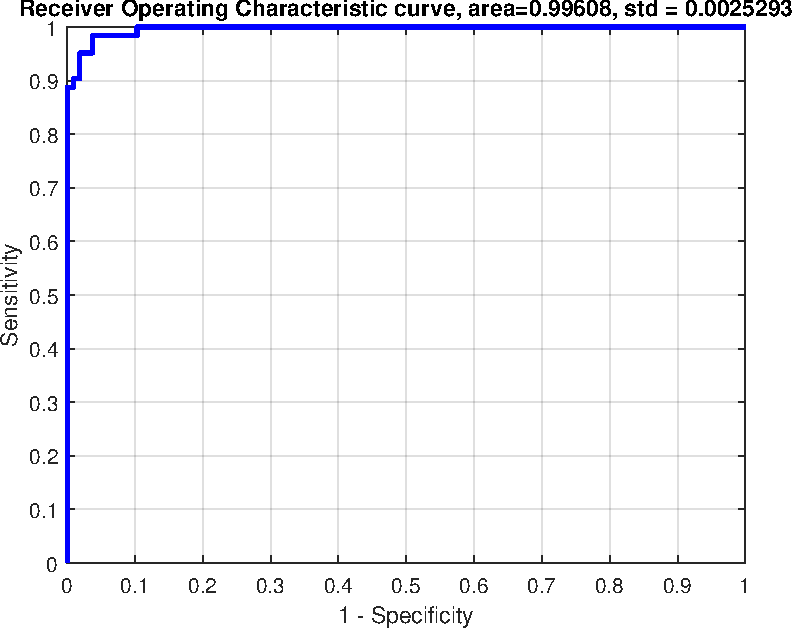
\includegraphics[width=\textwidth]{Assignment 1/figures/breast_linear_classifier_roc.pdf}
                \caption{Linear kernel}
                 \label{fig:breast_liner_roc}
             \end{subfigure}
             \hfill
             \begin{subfigure}[b]{0.3\textwidth}
                 \centering
                 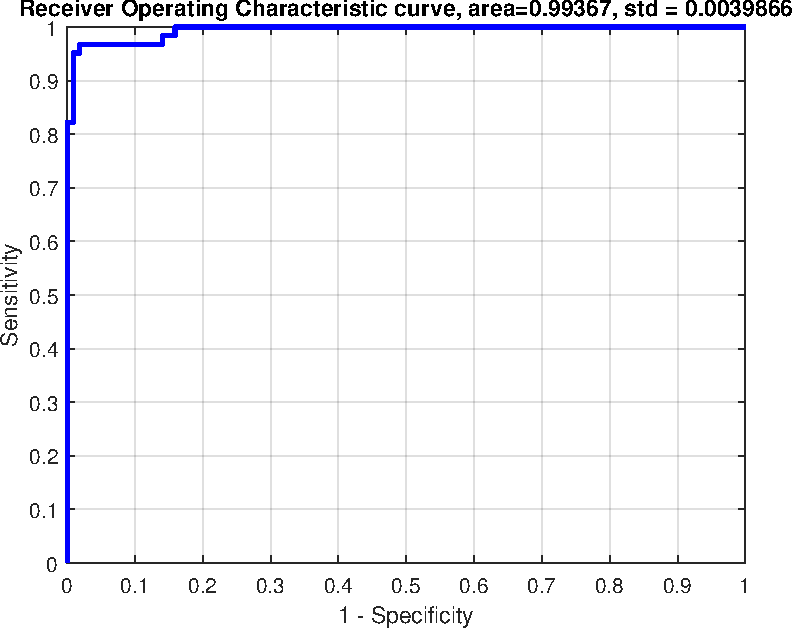
\includegraphics[width=\textwidth]{Assignment 1/figures/breast_rbf_classifier_roc.pdf}
                \caption{RBF kernel}
                 \label{fig:breast_rbf_roc}
             \end{subfigure}
             \hfill
             \begin{subfigure}[b]{0.3\textwidth}
                 \centering
                 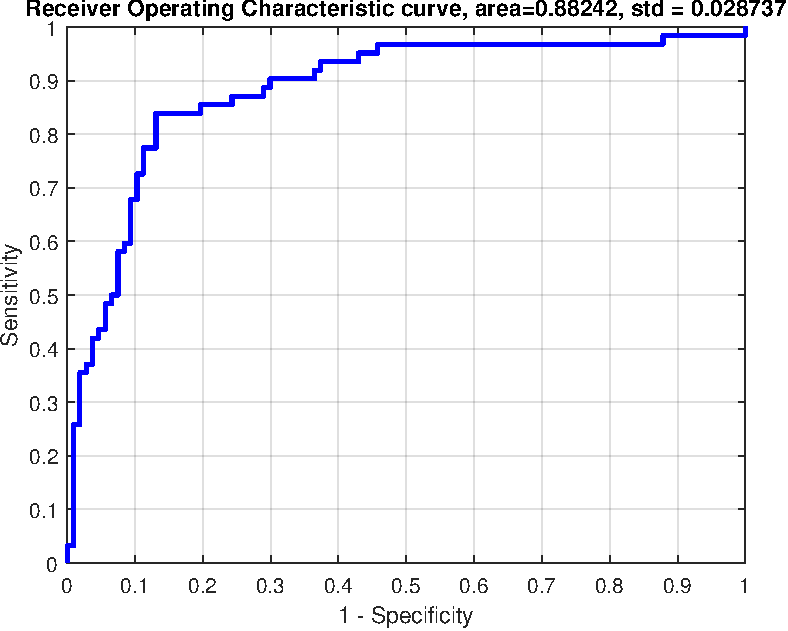
\includegraphics[width=\textwidth]{Assignment 1/figures/breast_polynomial_classifier_roc.pdf}
                \caption{Polynomial kernel}
                 \label{fig:breast_poly_roc}
             \end{subfigure}
            \caption{Binary classification results for the Breast Cancer dataset for Linear, RBF and Polynomial kernels tuned with the Simplex algorithm.}
            \label{fig:breast_cancer_overall}
        \end{figure}
        
    \subsection{Diabetes dataset}
        The Diabetes dataset consists of 8 features which are plotted in a t-SNE plot in figure \ref{fig:diabetes_dataset}. From the t-SNE plot it  can be see there is more overlap between the features than the Breast Cancer dataset, suggesting that a more nonlinear model such as a RBF kernel SVM would would be needed. However, since the dataset contains a high-dimensional input space, a linear kernel SVM would most probably also perform well for this dataset. 
        % Diabetes dataset
        \begin{figure}[H]
            \centering
            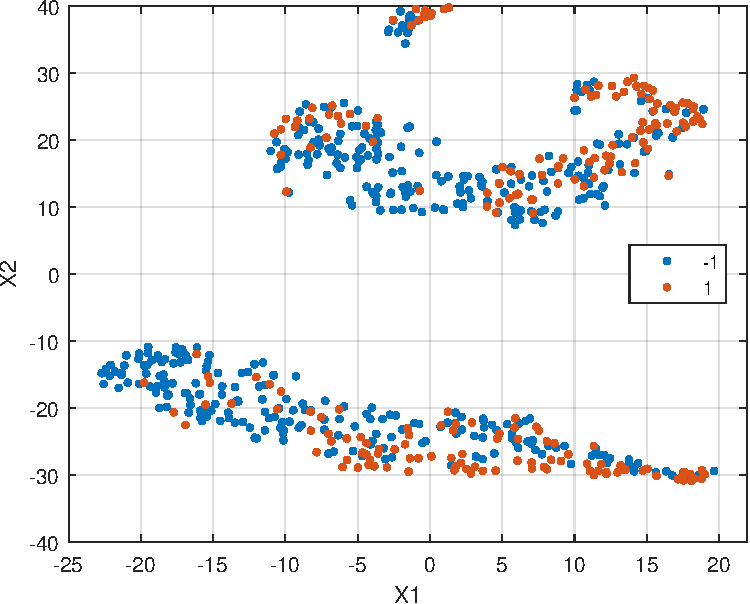
\includegraphics[width=0.450\textwidth]{Assignment 1/figures/diabetes_data.pdf}
            \caption{Diabetes dataset with shape $(600,8)$.}
            \label{fig:diabetes_dataset}
        \end{figure}
        
        Linear, RBF, and polynomial kernels were tested with Simplex-tuned hyperparameters over a  10-fold cross validation set. The results are shown in figure \ref{fig:diabetes_overall}. The best performing classified was the RBF kernel obtaining a ROC curve area of $0.8454$, however as suspected the linear kernel did equivalently well with an ROC curve area of $0.84449$. 
        
        % ROC curves for diabetes
        \begin{figure}[H]
             \centering
             
             \begin{subfigure}[b]{0.3\textwidth}
                 \centering
                 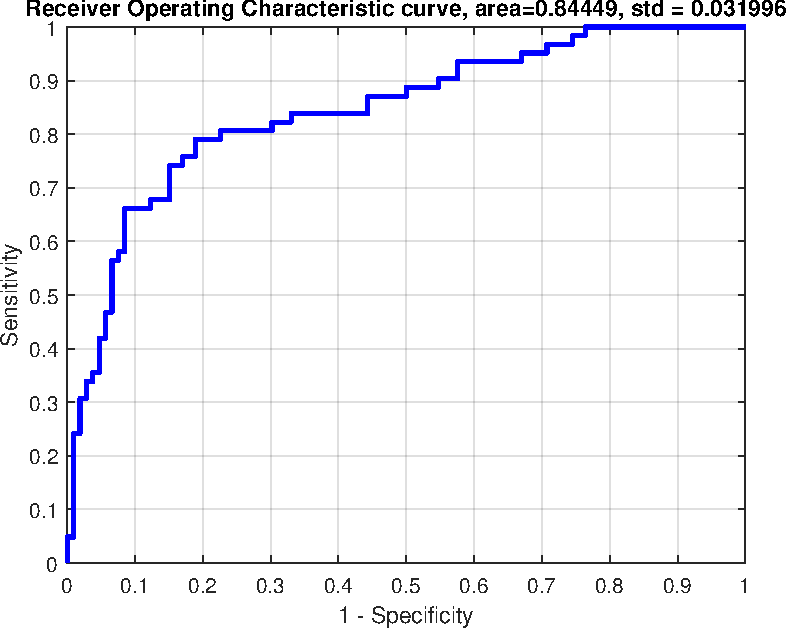
\includegraphics[width=\textwidth]{Assignment 1/figures/diabetes_linear_classifier_roc.pdf}
                \caption{Linear kernel}
                 \label{fig:diabetes_liner_roc}
             \end{subfigure}
             \hfill
             \begin{subfigure}[b]{0.3\textwidth}
                 \centering
                 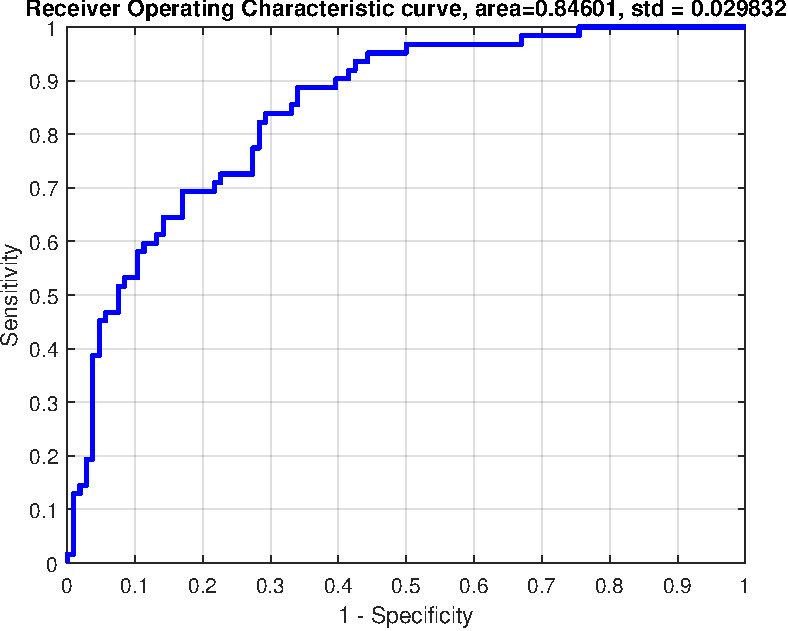
\includegraphics[width=\textwidth]{Assignment 1/figures/diabetes_rbf_classifier_roc.pdf}
                \caption{RBF kernel}
                 \label{fig:diabetes_rbf_roc}
             \end{subfigure}
             \hfill
             \begin{subfigure}[b]{0.3\textwidth}
                 \centering
                 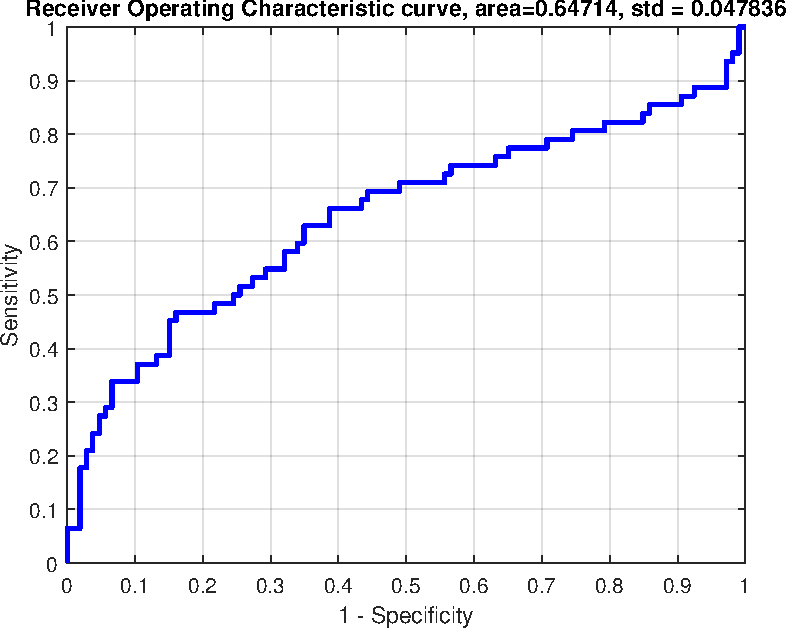
\includegraphics[width=\textwidth]{Assignment 1/figures/diabetes_polynomial_classifier_roc.pdf}
                \caption{Polynomial kernel}
                 \label{fig:diabetes_poly_roc}
             \end{subfigure}
            \caption{Binary classification results for the Diabetes dataset for Linear, RBF and Polynomial kernels tuned with the Simplex algorithm.}
            \label{fig:diabetes_overall}
        \end{figure}
        
\end{document}
